\subsection{Handwriting synthesis}
\label{sec:synthesis}

This subsection describes how a text is converted into pen paths in the style of a stored writer (functional units FU~2.7 and part of FU~2.5; requirements R1 and R3).
It takes the text, a style profile (Section~\ref{sec:styleprofile}), the x-height size $x_{\mathrm{mm}}$ in millimetres, 4\,mm by default, and a random seed, and returns a \emph{trajectory}: pen-down polylines in millimetres, $y$ upwards, origin at the first baseline.
Geometry stays in x-height units until one multiplication at the end, so one profile serves any pen size, and because the construction is random a search over several candidates (Section~\ref{sec:syn-search}) keeps the one that the text recogniser of Section~\ref{sec:textrec} and the stroke-normalised writer classifier of Section~\ref{sec:writerid} jointly prefer.

\subsubsection{Global quantities and glyph choice}

Let $\theta_{\mathrm p}$, $c$, $A$, $D<0$ and $g$ be the profile's slant, connectedness, ascender and descender reach and word gap, and $\lambda\in[0,1]$ the writer's legibility parameter, which is 0 for every writer in the delivered system because the key is missing from the stored profiles (Section~\ref{sec:styleprofile}): every formula below containing $\lambda$ must be read at $\lambda=0$ to judge what the submitted code does.
The synthesiser derives, by Equation~\ref{eq:syn-global},
\begin{equation}
\theta_{\mathrm{cap}}=45^\circ-19^\circ\lambda,\quad\sigma=\tan\!\bigl(\operatorname{clip}(\theta_{\mathrm p},\pm\theta_{\mathrm{cap}})\bigr)+\Delta_\sigma,\quad p_{\mathrm j}=\min(c,1),\quad L=(A-D+0.85)\,x_{\mathrm{mm}},
\label{eq:syn-global}
\end{equation}
Each quantity in Equation~\ref{eq:syn-global} has a specific job. The \emph{shear coefficient} $\sigma$ is the tangent of the writer's slant, so that multiplying a point's height by $\sigma$ and adding it to the horizontal coordinate leans the letter by that angle; this is the inverse of the de-slanting the builder applied when it stored the glyph upright. The calibration shift $\Delta_\sigma$ comes from Section~\ref{sec:syn-cal} and corrects the difference between the slant of individual letters and the slant of a whole assembled line. The angle is clipped to $\theta_{\mathrm{cap}}$ because a very steep lean makes adjacent letters collide. The \emph{join probability} $p_{\mathrm j}$ decides how often two neighbouring letters are connected, and the \emph{line pitch} $L$ is the baseline-to-baseline spacing in millimetres, which works out at 12.6\,mm for the default $A=1.7$, $D=-0.6$ and $x_{\mathrm{mm}}=4$\,mm.

The treatment of connectedness is a design decision worth stating, because the obvious approach failed. The stored connectedness $c$ is the measured fraction of adjacent letter pairs that the writer joins, so it is natural to read it as a threshold and join every pair when $c$ is above some value. Doing that joined \emph{every} pair for every writer above the threshold, which fused whole words into unbroken blobs and lost the irregularity that makes a hand look human. It is therefore used as a \emph{probability} instead: each pair is joined on an independent random draw below $p_{\mathrm j}$, so a writer who joins four pairs in five has roughly four joins in five but not the same four every time.

\paragraph{Choosing a glyph for each character.}
For each character the synthesiser works down a fallback chain and takes the first option that exists: the writer's own stored variants of that character, then a borrowed shape of the other case or of a visually similar character, then the \emph{anchor}, and finally a hand-designed skeleton or, failing everything, a blank. The chain exists because no writer's pages contain every character, so there must always be something to draw.

Among the writer's own variants the choice is random but weighted, by $w_i=(1+1.4i)^{-1}\exp[-((\mathrm{entryY}_i-\hat e)/0.45)^2]$ for rank $i=0,\ldots,4$, where the variants are ranked by $\mathrm{priorD}$ so that rank 0 is the most typical. The two factors do different things. The first falls off with rank, so a more typical variant is chosen more often but an unusual one is still chosen sometimes, which is what stops every instance of a letter on the page being identical. The second factor applies only when the letter is being joined to the previous one: $\hat e$ is the height at which the pen is currently leaving the previous letter, $\mathrm{entryY}_i$ is the height at which this variant begins, and the Gaussian penalises a mismatch between them. Choosing a variant whose entry height matches where the pen already is avoids a join that loops awkwardly up or down to meet it.

The \emph{anchor} is the legible fallback, and its role is to put a floor under how bad a letter can be. It is the writer's own medoid when that is clean enough, which keeps it in the writer's hand. When the medoid is itself malformed, the anchor is instead a hand-designed single-stroke skeleton, joined cursive for a connected hand and upright print otherwise, re-proportioned to the writer's own ascender and descender reach so that it does not sit at the wrong size among real letters. The print skeleton reads back at about 96\,\% character and 84\,\% word accuracy, which is clearer than any glyph derived from the data, and that is what makes it a usable floor. Table~\ref{tab:syn-const} in Appendix~\ref{sec:app-syn} gives the constant behind each of these choices with the reason for its value.

\paragraph{Trading style against legibility.}
The system has two goals that pull against each other. Requirement R1 asks for handwriting that resembles the writer, which argues for always using the writer's own letters, and it also asks for handwriting that can be read, which argues for replacing the writer's worst letters with something clearer. The parameter $\lambda$ is the single control that sets where a given writer sits between those two.

The obvious implementation would be to blend the two shapes geometrically, drawing a curve part way between the writer's glyph and the anchor. That is \emph{not} what is done, and the reason is that an average of two different pen strokes is usually not a valid letter at all: blending a one-stroke and a two-stroke form of the same character produces something neither legible nor characteristic. Instead $\lambda$ scales the \emph{probability} that a chosen variant is replaced by the anchor outright, so every letter drawn is always a real letterform, either the writer's or the anchor's. Equation~\ref{eq:syn-swap} gives that probability as a function of $\lambda$ and the variant's prior distance $d$ from Equation~\ref{eq:sty-prior}. The same $\lambda$ also lowers the slant cap in Equation~\ref{eq:syn-global}, since a reduced lean is the other thing that helps legibility.
\begin{equation}
P_{\mathrm{swap}}(\lambda,d)=\begin{cases}1&d\ge0.55,\\0&\lambda\le10^{-3},\\0.06\,\lambda&d\le0.12,\\\operatorname{clip}\bigl(\lambda\,(0.55+0.9\,b),0,1\bigr),\ b=\operatorname{clip}\bigl(\tfrac{d-0.12}{0.43},0,1\bigr)&\text{otherwise.}\end{cases}
\label{eq:syn-swap}
\end{equation}
The four cases of Equation~\ref{eq:syn-swap} implement three different policies, and the thresholds 0.12 and 0.55 on $d$ are what separate them. A variant further than $d=0.55$ from the cross-writer reference is replaced \emph{unconditionally}, whatever $\lambda$ says, because at that distance the shape is no longer recognisable as the character and keeping it would serve neither goal. A variant closer than $d=0.12$ is kept almost always, the replacement probability being only $0.06\lambda$, because a shape that close to the reference is already legible and replacing it would cost style for nothing. Between those two the probability rises linearly with $d$ through the interpolation variable $b$ and scales with $\lambda$, so a writer tuned to a high $\lambda$ has their marginal letters replaced and a writer tuned to zero does not. At $\lambda=1$ this gives 0.74 for $d=0.21$ and 0.99 for $d=0.33$. The second case makes $\lambda=0$ exact rather than approximate: below $10^{-3}$ the replacement is switched off entirely, so a writer tuned to zero keeps even their marginal letters, and only the unconditional case above $d=0.55$ still fires.

Measured over a design-stage probe, the resulting share of anchor glyphs ran from 0\,\% for writer 552 to 76\,\% for writer 151, which is the spread the parameter is there to produce: writer 151's hand is the most joined of the set and suffers most from being cut into letters, so it needs the most help, while writer 552's letters survive the process intact.
$\lambda$ is set per writer (Table~\ref{tab:sty-writers}) by an automatic search on a novel corpus followed by manual adjustment against the evaluation script; in the delivered system the mechanism is inert and every figure in this paragraph describes the tuned configuration only, as item~1 of Section~\ref{sec:syn-faults} sets out.
A geometric blend toward the anchor and a soft-archetype proposal appear only in the project notes and not in the delivered code.

\subsubsection{Placement, joins and randomness}

A chosen glyph $(x,y)$, in x-height units and upright, is placed at the pen position $(P_x,P_y)$ in millimetres by Equation~\ref{eq:syn-place},
\begin{equation}
X=P_x+(\ell+x+\sigma_g\,y)\,x_{\mathrm{mm}},\qquad Y=P_y+(y+\delta_g)\,x_{\mathrm{mm}},
\label{eq:syn-place}
\end{equation}
with the glyph's lead $\ell$, shear $\sigma_g$ and baseline drift $\delta_g$, which inverts the de-slanting of Equation~\ref{eq:sty-norm}; each glyph occupies a cell of its own advance with the ink starting after $\ell$, and the writer's own glyphs take the line shear $\sigma$ while anchor glyphs are capped more tightly.
Adjacent letters are joined when both are alphabetic, both are the writer's own glyphs or both the cursive anchor, and a random draw falls below $p_{\mathrm j}$; a print anchor is never joined through, and a joined run is one pen-down polyline, so the pen lifts only where the writer lifts.
One pseudo-random stream, seeded by the seed argument, supplies every draw, so the arguments fix the output completely: each glyph is rotated, scaled and translated a little and the baseline wanders as a bounded first-order walk, all scaled by one jitter amplitude $J$.
At $J=0.5$, the value the search uses, the jitter comes to a rotation of $1.1^\circ$, a scale change of 2.5\,\% and a translation spread below 0.05\,mm, enough to perturb a letter without changing its identity; Appendix~\ref{sec:app-syn} lists every constant of the placement, the joins, the randomness and the glyph choice with the reason for its value.


\paragraph{Style calibration.}
\label{sec:syn-cal}
A line of separate glyphs does not reproduce the line-level slant and reach of the real lines on its own: writer 150's ascenders came out about 7\,\% too tall and writer 551's slant about $9^\circ$ too steep.
A fixed probe sentence is therefore synthesised once per writer and size, at seed 17 with no jitter and measured with the estimators of Section~\ref{sec:styleprofile}, and three fixed-point iterations of Equation~\ref{eq:syn-cal} adjust the shear shift $\Delta_\sigma$ and the scale factors $K_A$, $K_D$ of the writer's tall and deep strokes until the probe matches the stored real-line values, ``ref'' being the stored value and ``got'' the probe value,
\begin{equation}
\Delta_\sigma\leftarrow\Delta_\sigma+\tan\theta_{\mathrm{ref}}-\tan\theta_{\mathrm{got}},\quad K_A\leftarrow\operatorname{clip}\Bigl(K_A\frac{A_{\mathrm{ref}}-1}{A_{\mathrm{got}}-1},0.5,1.6\Bigr),\quad K_D\leftarrow\operatorname{clip}\Bigl(K_D\frac{D_{\mathrm{ref}}}{D_{\mathrm{got}}},0.5,1.6\Bigr),
\label{eq:syn-cal}
\end{equation}
in which $\theta$ is the line slant of Equation~\ref{eq:sty-slant}, $A>1$ the ascender reach and $D<0$ the descender reach, the references being \texttt{slantMeasRef}, \texttt{ascMeasRef} and \texttt{descMeasRef} of Table~\ref{tab:sty-schema}, and the clip bounding each correction.
The factors are then applied as $y\leftarrow1+(y-1)K_A$ above the x-height line and $y\leftarrow yK_D$ below the baseline, and $\Delta_\sigma$ is added to the shear of Equation~\ref{eq:syn-global}.

\subsubsection{Best-of-$N$ search with joint scoring}
\label{sec:syn-search}

Single draws vary in quality, so the line is drawn $N$ times and the best candidate kept.
The score uses both judges, because selecting by text accuracy alone raised legibility but lowered writer identification for some writers (Table~\ref{tab:syn-evid}): the most legible draw need not be the most characteristic.
For a rendered candidate $I$, with $\hat y(I)$ the greedy CTC reading of Equation~\ref{eq:rec-greedy} and $y$ the intended text, the joint score is Equation~\ref{eq:syn-score},
\begin{equation}
a(I)=\max\Bigl(0,1-\frac{\mathrm{Lev}(\hat y(I),y)}{|y|}\Bigr),\quad w(I)=\mathrm{softmax}\bigl(f_{\mathrm{wid}}(I)\bigr)_{a^\star},\quad S(I)=\frac{2\,a(I)\,w(I)}{a(I)+w(I)},
\label{eq:syn-score}
\end{equation}
where $\mathrm{Lev}$ is the Levenshtein distance of Equation~\ref{eq:rec-lev}, $f_{\mathrm{wid}}$ the shape classifier after stroke normalisation (Section~\ref{sec:wid-strokenorm}), $a^\star$ the target writer, and $S=0$ if $a+w\le10^{-9}$.
The harmonic mean is dominated by the smaller term, so a candidate cannot win on one criterion while failing the other, and $w$ is a probability rather than a hit-or-miss flag.
Figure~\ref{fig:syn-search} is the control flow of the two loops that use it.

The search has two loops.
In the first, for $k=0,\ldots,N-1$, it synthesises a candidate with seed $\mathrm{base}+977k$ and $J=0.5$, renders it at 0.085 x-heights and 18 pixels per millimetre, computes $S$, keeps the candidate if it beats the best so far, and leaves the loop once the best reaches 0.99 or $k=N-1$.
The second is the \emph{repair} loop, which exits straight to the output once the best is at or above 0.995 or three rounds have run; otherwise each round starts from the best candidate so far, forced-aligns the intended text to the recogniser output on its image (Equation~\ref{eq:sty-viterbi}), scores each non-space character by its mean own-class log-probability over its own frames, taken as $-10^9$ if the path never visits it, pins the two worst unpinned characters to the anchor, re-synthesises the \emph{whole} line with seed $\mathrm{base}$, judges it, and accepts only if the joint score strictly exceeds the best so far, the round ending either way.
Re-using seed $\mathrm{base}$ makes the repair a fresh draw with pins rather than a patch of the winner, and judging it jointly rejects a repair that fixes a letter but makes the line look like another writer, whereas a text-only search with a plain repair that accepts on text score alone was measured to cost writer identification (Table~\ref{tab:syn-evid}).

\begin{figure}[!htbp]
\centering
\begin{tikzpicture}[node distance=3.5mm and 6mm]
\node[w3io] (in) {text, profile, writer $a^\star$, seed base, $N$};
\node[w3box,below=of in] (syn) {synthesise candidate $k$\\seed $\mathrm{base}+977k$, $J=0.5$};
\node[w3box,below=of syn] (ren) {render at 0.085 x-heights, 18\,px/mm};
\node[w3dark,below=of ren] (sco) {score $S$ by Equation~\ref{eq:syn-score}\\recogniser $a(I)$, classifier $w(I)$};
\node[w3dec,below=4.5mm of sco] (better) {$S>S_{\mathrm{best}}$?};
\node[w3store,right=14mm of better] (keep) {keep as best};
\node[w3dec,below=5mm of better] (loop) {$S_{\mathrm{best}}\!\ge\!0.99$\\or $k\!=\!N\!-\!1$?};
\node[w3dec,below=5mm of loop] (done) {$S_{\mathrm{best}}\!\ge\!0.995$\\or 3 rounds?};
\node[w3box,below=of done] (align) {forced-align text to the best image\\(Equation~\ref{eq:sty-viterbi}); score each character\\by its mean own-class log-probability};
\node[w3box,below=of align] (pin) {pin the two worst unpinned characters\\to the anchor; re-synthesise the whole\\line at seed base; render; score};
\node[w3dec,below=4.5mm of pin] (acc) {improved?};
\node[w3io,below=5mm of acc] (out) {best trajectory};
\draw[w3arr] (in) -- (syn);
\draw[w3arr] (syn) -- (ren);
\draw[w3arr] (ren) -- (sco);
\draw[w3arr] (sco) -- (better);
\draw[w3arr] (better) -- node[w3lab,above]{yes} (keep);
\draw[w3arr] (better) -- node[w3lab,right]{no} (loop);
\draw[w3arr] (keep.south) |- (loop.east);
\draw[w3arr] (loop) -- node[w3lab,right]{yes} (done);
\draw[w3arr] (loop.west) -- node[w3lab,above,pos=0.3]{no, $k\!\leftarrow\!k\!+\!1$} ++(-16mm,0) |- (syn.west);
\draw[w3arr] (done) -- node[w3lab,right]{no} (align);
\draw[w3arr] (align) -- (pin);
\draw[w3arr] (pin) -- (acc);
\draw[w3arr] (acc.west) -- node[w3lab,above,pos=0.35]{either way} ++(-14mm,0) |- (done.west);
\draw[w3arr] (done.east) -- node[w3lab,above,pos=0.4]{yes} ++(16mm,0) |- (out.east);
\node[w3group,fit=(syn)(ren)(sco)(better)(keep)(loop),label={[w3lab]above right:best-of-$N$ loop}] {};
\node[w3group,fit=(align)(pin)(acc),label={[w3lab]below right:repair loop, at most 3 rounds}] {};
\end{tikzpicture}
\caption{Control flow of the candidate search of \texttt{SynthesizeJointBestOf}. The upper loop draws $N$ candidates and keeps the one with the highest joint score $S$ of Equation~\ref{eq:syn-score}; the lower loop attempts at most three repairs, each a fresh draw of the whole line with the two weakest characters pinned to the anchor, and accepts one only when $S$ strictly improves, so a repair that fixes a letter at the cost of the writer's identity is rejected. Both judges score the same rendered ink, the classifier after the stroke normalisation of Section~\ref{sec:wid-strokenorm}.}
\label{fig:syn-search}
\end{figure}

$N$ is 6 as the function default, 14 for the design-stage measurements, 20 as the web default and 30 in the official evaluation script, and the search cost is linear in it by Equation~\ref{eq:syn-cost}.
The cost is entirely judge-bound: synthesising a candidate takes 11 to 16\,ms against 0.5 to 4\,s to score it, and within that score the dominant term is thinning the full-resolution render rather than either network, so the whole search at $N=14$ took 23 to 137\,s on the laptop.
That is where any optimisation must go, and it is also why $N$ rather than the construction sets the reproduction time of requirement R3.
Appendix~\ref{sec:app-syn} resolves Equation~\ref{eq:syn-cost} into its measured terms for three writers and gives the order-statistics argument for the diminishing return from raising $N$.


\subsubsection{Design-stage measurements of the synthesiser}

Table~\ref{tab:syn-evid} lists the measurements that motivated the design, taken over six novel sentences, two seeds and ten writers, so 12 lines per writer and one misjudged line moves a writer's rate by 8.3 percentage points, together with the final system for comparison.
Items~2 and~3 of Section~\ref{sec:syn-faults} state why every row after the search was introduced is circular, and the non-circular reference is the recogniser on \emph{real} held-out handwriting of the same writers, 89.4\,\% character and 70.8\,\% word accuracy (Table~\ref{tab:rec-data}, with possible training overlap).

\begin{table}[!htbp]
\centering
\fontsize{8}{9.6}\selectfont
\setlength{\tabcolsep}{4pt}
\begin{tabularx}{\linewidth}{|X|c|c|}
\hline
\textbf{Stage} & \textbf{Writer ID, direct / G-code (\%)} & \textbf{Char.\ acc., direct / G-code (\%)} \\
\hline
Plain synthesis after label and glyph fixes & 79.2 / 80.0 & 75.9 / 76.3 \\
+ per-writer $\lambda$ & 83.3 / 86.7 & 77.2 / 77.8 \\
Text-only best-of-$N$ with plain repair & 76.7 / 73.3 & 83.8 / 82.7 \\
Joint best-of-$N$, $N=6$ & 92.5 / 92.5 & 79.9 / 79.6 \\
Joint best-of-$N$, $N=14$ & 97.5 / 95.8 & 81.6 / 81.4 \\
\hline
Final system, 13 writers, 3 sentences, $N=8$ & 92.3 / 89.7 & 79.2 / 79.2 \\
Final system, 13 writers, 6 sentences $\times$ 2 seeds, $N=30$ & 80.1 / 78.8 & 82.2 / 82.5 \\
\hline
Matching comparison: the writers' own handwriting of the same words & not applicable & 89.0 / --- \\
Matching comparison: the system's synthesis of those same words & not applicable & 81.6 / --- \\
\hline
\end{tabularx}
\caption{Measurements that motivated the design (upper block) and the final system (lower blocks). ``G-code'' means converted to G-code and read back (Section~\ref{sec:gcode}). Only the two matching-comparison rows are independent of the search and so the figures to trust; the rest, and the unavailability of the per-writer $\lambda$ gain, are qualified by items~1 to~3 of Section~\ref{sec:syn-faults}.}
\label{tab:syn-evid}
\end{table}

On the matching comparison of identical words synthesis costs 7.4 percentage points of character accuracy, 89.0\,\% against 81.6\,\%, and divides word accuracy by more than 1.5, 70.5\,\% against 46.7\,\%, which locates the loss in spacing and word boundaries rather than in letterforms.
Figure~\ref{fig:res-e2e} shows the per-writer breakdown and Figure~\ref{fig:syn-lines} one candidate each for a print and a joined hand.

\begin{figure}[!htbp]
\centering

\includegraphics[width=0.95\linewidth]{Figures/w3_synth_150.png}\\[1pt]
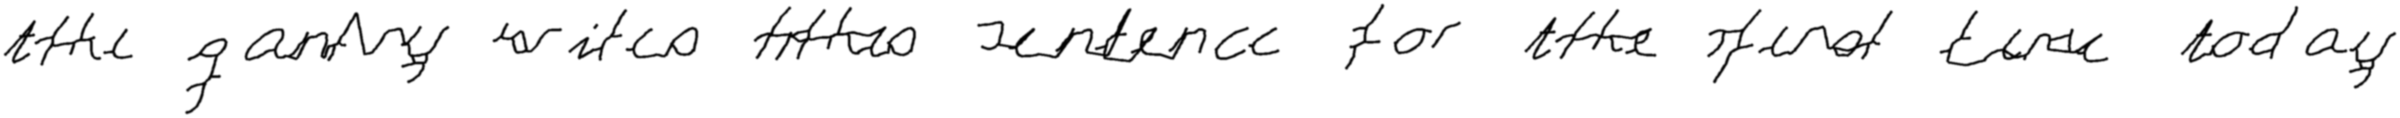
\includegraphics[width=0.95\linewidth]{Figures/w3_synth_153.png}
\caption{Synthesised line ``The gantry writes this sentence for the first time today'' for writer 150 (upper, printed hand; read back with three small errors) and writer 153 (lower, joined hand; read back as ``the garoby writes tttas senkence for tthe furst tuse today''), one seed and candidate each, rendered from the trajectory of an end-to-end run; the $N$ of that run was not recorded.}
\label{fig:syn-lines}
\end{figure}

\subsubsection{Design alternatives and justification}

A recurrent sequence generator with attention and mixture-density output needs on-line pen data, hundreds to thousands of lines per writer, whereas only 47 to 130 scanned lines per writer exist (Table~\ref{tab:sty-writers}); a from-scratch version trained on skeleton-derived strokes learned slant, roundness and connectedness but no legible letters and was rejected.
Adversarial and diffusion generators need less data through pre-training, but they emit a raster that needs the same thinning to vectorise, size, slant and spacing cannot be controlled as numbers, and a trial took 35 to 45\,s per line against 3 to 8\,s for glyph synthesis, so they were parked.
The glyph library needs about nine pages per writer and no training, outputs pen strokes directly, exposes size, slant, joins and gap as explicit numbers and has a traceable fallback for every glyph; synthesis itself costs about 15\,ms, so only the optional search is expensive, which suits a single-board computer without an accelerator, and the one weakness is joined hands, whose joins are lost by cutting.

\subsubsection{Known faults and limitations}
\label{sec:syn-faults}

\begin{enumerate}\setlength{\itemsep}{0pt}\setlength{\parskip}{0pt}
\item \emph{The legibility mechanism is inert as submitted.} \texttt{legibilityLambda} is absent from all thirteen stored profiles and \texttt{SynthesizeJointBestOf} defaults it to zero, so $\lambda=0$ on the live path: the second branch of Equation~\ref{eq:syn-swap} fires for every glyph below $d=0.55$, the \emph{only} substitutions left are the unconditional ones at $d\ge0.55$, and the cap stays at its widest, $\theta_{\mathrm{cap}}=45^\circ$. Every $\lambda$-dependent figure above, including the 0 to 76\,\% anchor share, describes the tuned configuration and \emph{not} the delivered one, and the outstanding tuner item of Section~\ref{sec:sty-faults} applies to all of them.
\item \emph{Every figure after the search was introduced is the opinion of the very networks that selected the output.} The search loads the same weight files as the measurement, so a best-of-$N$ search necessarily raises the score by which it is judged; the values show that the pipeline can satisfy its two judges, not that a human reader or an independent recogniser would agree.
\item $\lambda$, the anchor threshold and $N$ were tuned on the same sentences that Section~\ref{sec:results} measures.
\item The calibration of Equation~\ref{eq:syn-cal} measures both sides with the same estimator, so the agreement of slant and reach it achieves is partly self-fulfilling and is not independent evidence.
\item The repair pass updates the pin set only on acceptance, so after a rejection the next round re-synthesises an identical candidate and the remaining rounds are wasted work; in three probe runs, writers 150, 153 and 551 at $N=14$, no repair was accepted at all.
\item Three design-stage figures have no surviving raw log: the 80.5 against 75.5\,\% variant-restriction probe, the anchor-share probe, and the print skeleton's 96 and 84\,\% read-back, which exists only as a code comment.
\mustdo{the corresponding read-back accuracy of the \emph{cursive} skeleton. An earlier draft quoted about 89\,\% for it; that figure matches no comment or log in the delivered code and has been withdrawn rather than left standing as a measurement.}
\item Writers 151 and 552, the two most joined hands, reach only 53 and 56\,\% character accuracy through G-code against about 84\,\% for the other eleven, the clearest limitation of the exemplar approach.
\end{enumerate}
